\section{Aufbau}
\label{sec:Aufbau}
Eine Skizze des Aufbaus ist in Abbildung \ref{fig:aufbau} zu sehen.
Die Probe befindet sich im Inneren des Rezipienten.
Sie ist mit einer Heizspirale umwickelt, als Energiezulieferer.
Der Rezipient kann mit der Vakuumpumpe geleert und mit Helium gefüllt werden.
Das Helium hat den Vorteil gegenüber Luft, dass es bei der Siedetemperatur von
Stickstoff $\left[\SI{77}{\kelvin}\right]$ gasförmig bleibt und nicht wie Luft kondensiert.
Dies ist wichtig, da der Rezipient während der Messung in einem Dewargefäß,
welches mit eben flüssigem Stickstoff gefüllt ist, ist.

Die Messung der Temperatur erfolgt mit zwei \enquote{Pt-100-Messwiderständen},
eines für die Probe, eins für das Gehäuse, abgelesen werden sie an zwei Ohmmetern.

Die Heizspule wird mit eineem Konstantstromgerät versorgt, zusätzlich gibt es eine
Gehäuseheizung.
\begin{figure}
  \centering
  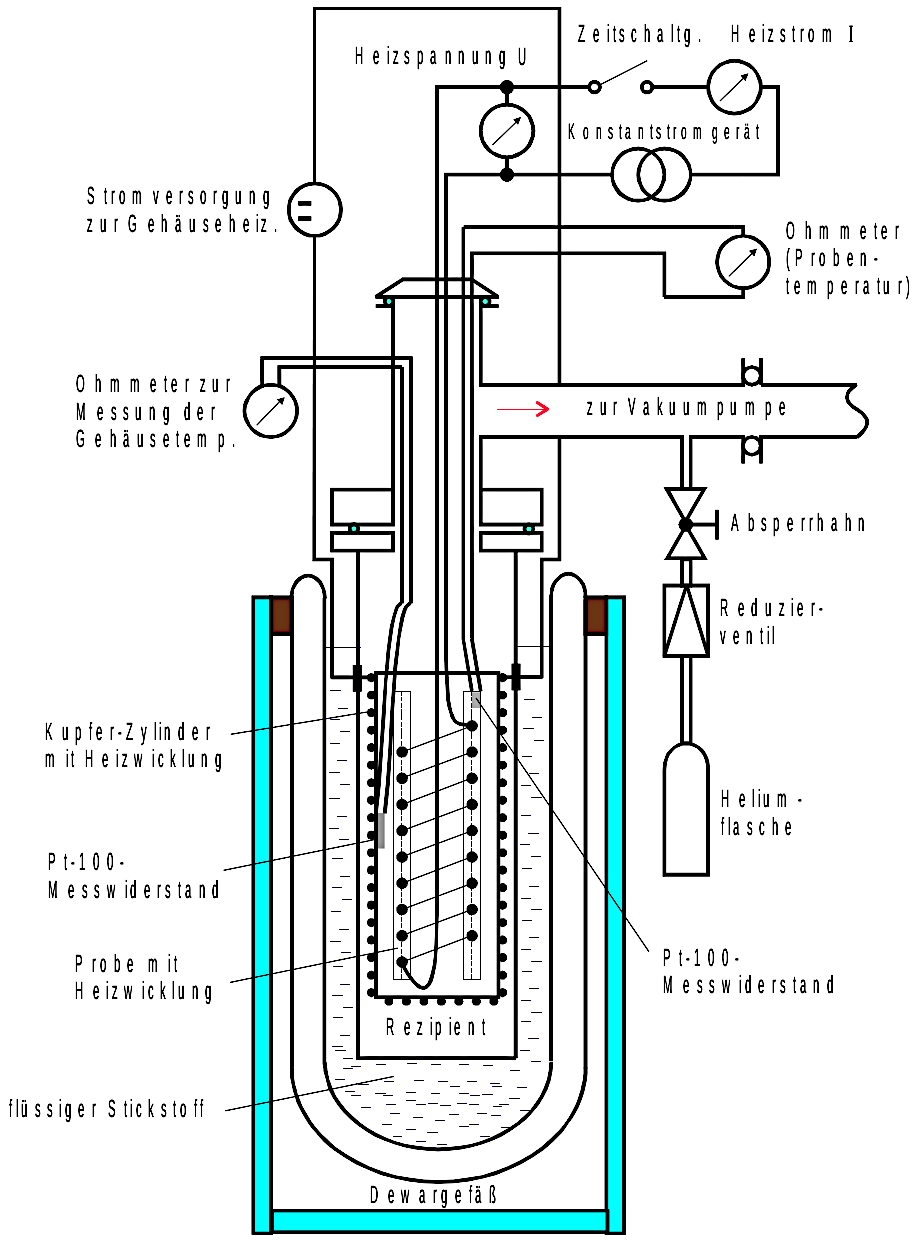
\includegraphics[height=0.6\textheight]{images/aufbau.png}
  \caption{Skizze der Versuchsapperatur, \cite{anleitung}.}
  \label{fig:aufbau}
\end{figure}

\section{Durchführung}
\label{sec:durchfuehrung}
Zu Beginn der Messung wird der Rezipient evakuiert und anschließend mit Helium gefüllt.
Dann wird das Dewargefäß mit flüssigem Stickstoff gefüllt und gewartet bis Gehäuse-
und Probentemperatur bei ungefähr $\SI{80}{\kelvin}$ sind. Während des Einkühlvorgangs
muss eventuell stickstoff nachgefüllt werden, zudem ist zu bemerken, dass die Probe
langsamer kühler wird als das Gehäuse. Ist die Zieltemperatur erreicht, wird mit
der Vakuumpumpe der Druck minimiert (bei uns hat die Druckmessung nicht funktioniert,
sodass mit Erfahrungswerten der Laufzeiten gearbeitet wurde).
In der eigentlichen Messung wird die Probe mit einem Strom von circa
$\SI{165}{\milli\ampere}$ bei einer Spannung von $\SI{17.64}{\volt}$
geheizt. Die Werte für das Gehäuse sind $I_{\text{G}} = \SI{4}{\ampere}$ und
$U_{\text{G}} = \SI{5}{\volt}$. Es muss darauf geachtet werden, dass der
Temperaturunterschied nicht zu groß ist, $\Del{R} \leq \SI{1}{\ohm}$.
Bis zu einem gemessenen Widerstand von $\SI{56}{\ohm}$ werden alle
$\SI{150}{\second}$ die Widerstände, Ströme und Spannungen notiert,
danach alle $\SI{300}{\second}$.
Die Ströme werden während der Messung verändert,
wenn die Differenz der Temperaturen zu groß wird.
